\cleardoublepage
\backmatter
\chapter{中德文化补充说明}
    在这里我们将通过服饰、饮食、体育、工作、交通、艺术和卫生这七个角度,探索中德两国的文化差异,
领略两国各异的
人文风情和生活方式。

\section{服饰}
    传统服饰是反应过去时代文化和人们对地域环境影响下形成的文化标志之一。在历史的长河中,
各个地域、各个民族都形成了风格迥异的传统服装。在人类近代化的发展潮流中,政治、经济、文化都发生了日新月异的变化,
这些变化都会对服装的演变产生深刻的影响。如果我们仔细观察中德两国传统服饰现代化演变的过程,可以发现这样一个显著的特征,
传统服饰由原来的拘谨、保守、呆板,逐渐向美观、适体、方便、平民化转变。在这里,我将以中徳两国具有代表性的女性传统服装为例,
通过介绍它们在近代化过程中的演变,来体现两国在服装上面迥异的文化。

\subsection{旗袍的前身——旗装}
\begin{figure}[htb]
\centering
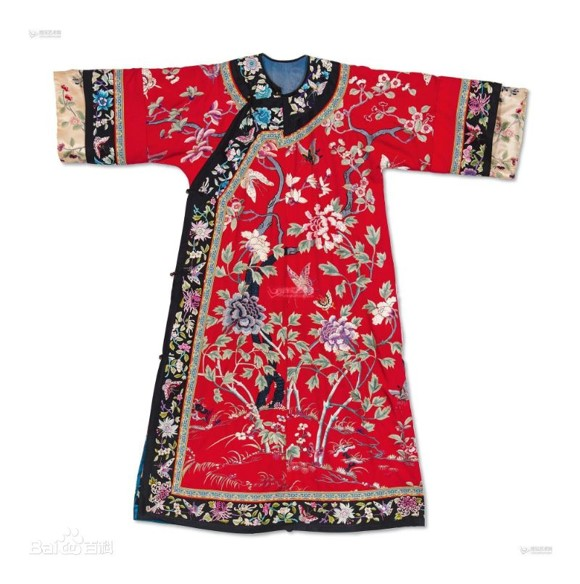
\includegraphics[width=0.6\linewidth]{Qizhuang}
\caption{清代旗装}
\end{figure}

    对于旗袍的来源,历来都有许多争议,比较主流的观点是现代旗袍改良自清代旗装。在浓厚的清朝封建礼教氛围中,妇女不可能如图现代一般将身体的曲线表现出来,否则会被视为不符合道德。因此清代旗装的裁制一直采用直线,衣身宽松,使女性身体的曲线不能外露,在现在看来,有点笨重和土气。 

    在色彩搭配方面,旗装色彩鲜艳复杂,喜欢使用高对比度的色彩搭配,并在衣身上绣有花、鸟、兽等图案,寓意吉祥,其中黄色是皇家专用的颜色,平民是禁止使用的。 
    
\subsection{旗袍的发展与流行}
\begin{figure}[htb]
\centering
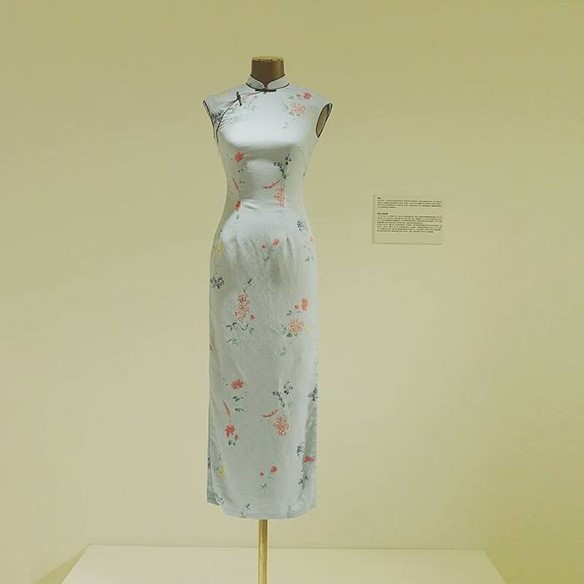
\includegraphics[width=0.6\linewidth]{Qipao}
\caption{现代旗袍}
\end{figure}

    1840年后进入近代,西洋文化侵袭着清朝的本土文化,服装也在开始发生变革。流行于二十世纪20年代的旗袍,是在民国妇女在穿着中吸收西洋服装对的式样,由传统的中国袍服不断改进而定型的。当时并没有专业服装设计机构,所以人民的服饰式样各不相同,在时代风尚的影响下不断变化。 

    从20世纪20年代至40年代末,中国旗袍风行了20多年,款式几经变化,领口的设计吸收了西式的特点,采用了当时时髦的样式,袖子也有原来的长袖改为了短袖,衣身变得更适体了,这时旗袍造型纤长,与欧洲流行的女装轮廓相吻合,让女性的体态和曲线美充分地体现出来了。 

\subsection{旗袍背后的文化内涵}

    旗袍的发展充分体现了当时妇女勇敢寻求思想上的解放,争取平等权利,反抗来自封建礼教的压迫,追寻独立自主的进步思想 。旗袍的发展历史不仅是中国服饰史的的一部分,也是中国近代化的一个标识之一。

    同样的,来自德国的传统女性服装Dirndl(德式连衣裙)也经过了一系列的改良和发展,至今仍然保留着旺盛的生命力。

\subsection{德式连衣裙的前身}
\begin{figure}[htb]
    \centering
    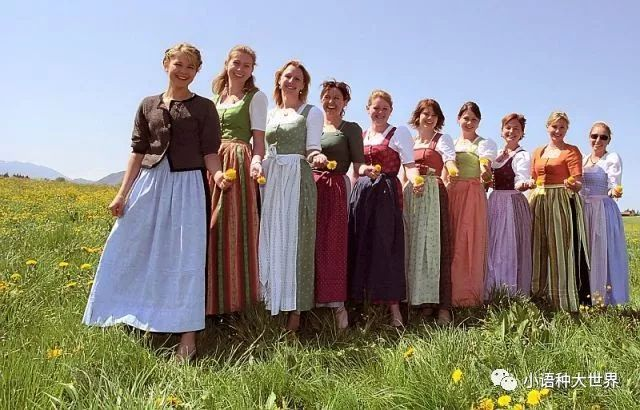
\includegraphics[width=0.6\linewidth]{alter Dirndl}
    \caption{老式Dirndl}
\end{figure}

    Dirndl是德国巴伐利亚地区和奥地利的一种传统的女性裙装。“Dirndl”原义指的是年轻姑娘,如今则为这类女性传统裙装统称。Dirndl起源于劳动妇女的工作服,材料为棉、亚麻、真丝或羊绒,颜色朴素沉静。 

    一套完整的Dirndl由四部分组成,Dirndl一般由这几个部分组成:衬衣或衬裙、紧身马甲、高腰半身裙和围裙。以前的衬衣的袖子一般都会长至肘部,“密封性"也相对较高——通常为方领或弧型领,也有长至脖子下方的,传统的半身裙也长至脚踝。 

\subsection{德式连衣裙的流行与发展}  
\begin{figure}[htb]
    \centering
    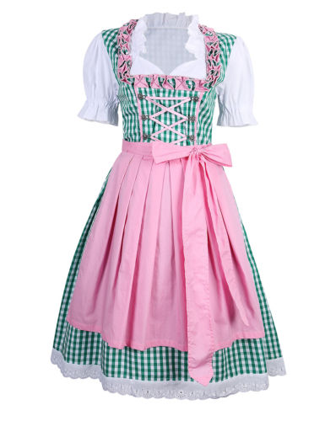
\includegraphics[width=0.6\linewidth]{neuer Dirndl}
    \caption{现代Dirndl}
\end{figure}

    随着时间的推移,服饰的发展总是趋于多元化,变得更加开放与活泼。十九世纪七八十年代的时候,城市的上流社会中有那么一群酷爱清凉一夏的人,这种轻便的田园夏装在她们之间得以流行。在一战后的经济困难时期,Dirdln彻底火了起来。因为比起那些做工精细、奢华昂贵的传统女性服装,它朴实无华又价格低廉,满足了那时广大女性的需求。

    在德意志第三帝国时期,纳粹执政党特别推崇德国传统服装。Gertrud Pesendorfer反对天主教的保守,主张在传统价值观念的框架里进行传统服饰的创新。Pesendorfer宣称,要将德国传统服饰从外来时尚艺术的影响中解放出来而使传统文化的根本重现时尚舞台。在这种情况下,Dirndl的袖子变得越来越短,衣领也变得越来越大,裙子也比原来变短了,Dirndl逐渐朝着现代服饰的方向演变。 

    如今,主要在德国南部和一些阿尔卑斯山地区,每逢集市、乡村地区的教堂落成典礼纪念日的年市或是盛大的民族节日人们还会穿着这种传统服饰。比如在盛大的慕尼黑十月啤酒节上,女士会穿上上鲜艳的Dirndl,胸前的设计突出了德国女人丰满的身材,腰间系的围裙又体现出德国女人窈窕的曲线,短短的泡泡袖设计在注重漂亮的同时,也很实用。 

\subsection{德式连衣裙上的文化内涵}  
     围裙,这块布真是充分显示出巴伐利亚妇女吃苦耐劳的品质,在十九世纪,奥地利人可是将之称为Dirndlgewand(女仆装扮)。不过,这块布可不仅仅是为了劳动而存在,它还包含着各式各样的个人信息,这在保守的时代可是相当重要:比如,围裙在左边打结,说明这位女性仍单身,当地有这样的说法:“Schleife links, Glück bringt’s!(左边系结,幸运到来)”。这样一来,单身男性就很容易分辨哪位窈窕淑女可以多加关注并有机会追求了。围裙在右面打结,表示这位女性已名花有主了。如果围裙结系在中间,说明这位女性的个人状况不确定(如下几种可能都有:处女、因为家庭原因而无法作出决定,或是自己想不清楚正在左右摇摆……)。如果围裙在身后打结,则只有两种可能:服务员或丧偶。 

\subsection{结语}  
    通过以上介绍,想必你们一定对旗袍和德式连衣裙有了基本的认识。旗袍和德式连衣裙既随着时代的发展不断变化,也保留了自己的传统和民族的特质,它们是新、旧时代交替的缩影。



\section{饮食}
     饮食文化涉及到食源的开发与利用、食具的运用与创新、食品的生产与消费、餐饮的服务与接待、餐饮业与食品业的经营与管理,以及饮食与国泰民安、饮食与文学艺术、饮食与人生境界的关系等,深厚广博。其具有风味多样,四季有别,注重情趣等特点。对于每一个学生来说,来到一个陌生的国家,饮食问题是非常重要的。为了帮助中德学子了解两国饮食文化,本文主要根据常见的饮食习俗来介绍。

\subsection{饮食文化简介}
    饮食本是人类最基本的活动,但若将问题提到为什么吃、怎么吃的层次,它就体现为一种意识或观念了。在饮食观念上,中西方有着明显的差异。

\subsection{中德——饮食文化}
    西方是一种理性的、讲求科学的饮食观念。他们强调饮食的营养价值,注重食物所含蛋白质、脂肪、热量和维生素的多少,而不追求食物的色、香、味、形的完美。 

    中国人的饮食强调感性和艺术性,追求饮食的口味感觉,而不注意食物的营养成份,多从“色、香、味、形、器”等方面来评价饮食的好坏优劣,追求的是一种难以言传的意境。简单地说,中国人吃的是口味。“味”,是中国饮食的魅力所在。中国人饮食的目的,除了果腹充饥,同时还满足对美味的渴望,带来身心的愉悦。

\subsection{中国的饮食习俗}
    中国人的饮食强调感性和艺术性,追求饮食的口味感觉,多从“色、香、味、形、器”等方面来评价饮食的好坏优劣,追求的是一种难以言传的意境。简单地说,中国人吃的是口味。“味”,是中国饮食的魅力所在。中国人饮食的目的,除了果腹充饥,同时还满足对美味的渴望,带来身心的愉悦。

\subsection{传统的中国美术——艺术}
    中国在追求食物的口味的同时,也追求食物的美感。通常会把食物雕刻成龙凤等动物的形状,或者仙桃,花朵等果实的形状。

    对食材的雕刻在中国是一门艺术,它有着自己的重要含义。龙和凤凰在中国代表着吉祥如意,而仙桃等代表着长寿。 

    长寿面是中国饮食文化的一种典型代表食物。老人在过生日时会吃这种面条,一碗面就一根面条,但是这根面条非常长,代表着祝福老人长命百岁。 

    \begin{figure}[htb]
        \centering
        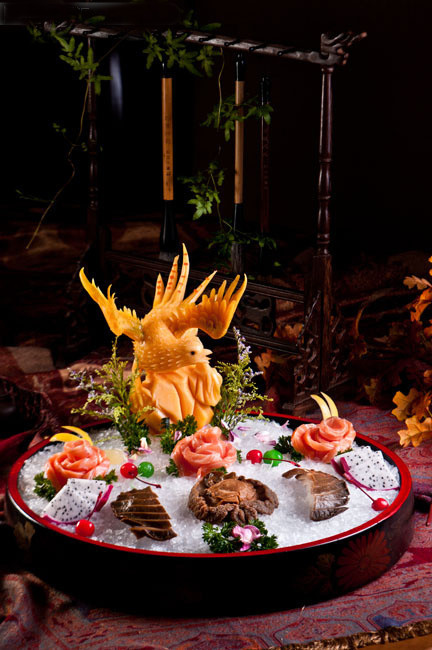
\includegraphics[width=0.6\linewidth]{caidiao}
        \caption{菜品雕刻}
    \end{figure}

\subsection{中国餐厅的饮食文化}
\item 中国餐厅是没有小费的。 
\item 一般用餐开始时间:17点到21点,持续1-2小时。 
\item 喝不重要,餐前一般会提高免费的茶水。 
\item 所有菜肴都很多。 
\item 用餐是使用筷子。 
\item 没有盐和胡椒调味。

\begin{figure}[htb]
    \centering
    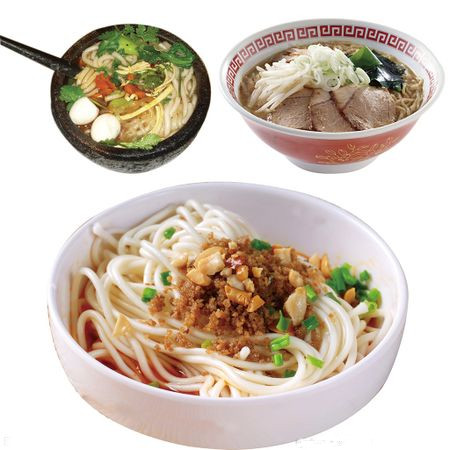
\includegraphics[width=0.6\linewidth]{noodle}
    \caption{面食}
\end{figure}

\subsection{德国的饮食习俗}
    西方是一种理性的、讲求科学的饮食观念。他们强调饮食的营养价值,注重食物所含蛋白质、脂肪、热量和维生素的多少,而不追求食物的色、香、味、形的完美。

\subsection{德国——圣诞节美食}
    下面以德国的圣诞节为例。在圣诞节时,德国人经常吃土豆沙拉,家禽或香肠。

    \begin{figure}[htb]
        \centering
        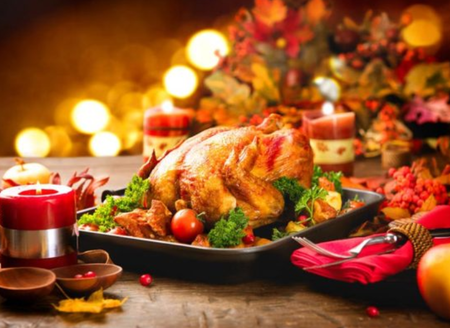
\includegraphics[width=0.6\linewidth]{christmas}
        \caption{圣诞美食}
    \end{figure}  

\subsection{德国——耶稣受难日}
    耶稣受难日德国人的食物是鱼或清淡的素食。 

    \begin{figure}[htb]
        \centering
        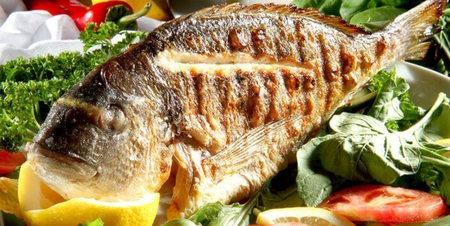
\includegraphics[width=0.6\linewidth]{fish}
        \caption{鱼}
    \end{figure}  

\subsection{德国——餐厅饮食文化}

\item 小费总额的2€至10% 
\item 开始吃饭的会议:19-20小时,2-3小时 
\item 喝重要 
\item 每个人都下令自己的法庭 
\item 餐具 
\item 调味盐和胡椒调味。

\begin{figure}[htb]
    \centering
    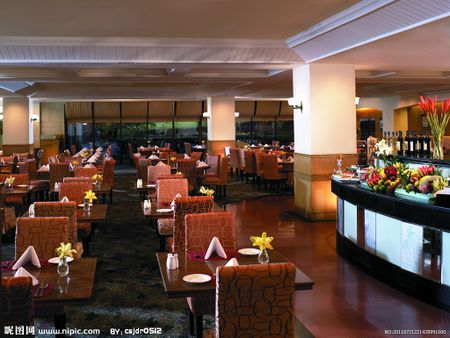
\includegraphics[width=0.6\linewidth]{restaurant}
    \caption{德国餐厅}
\end{figure} 



\section{体育}
    体育是一种精神,他代表了一个民族的勇气,坚强和毅力。体育可以磨练一个人的精神品质,这对我们无论在各个方面都很重要。精神品质是一个人的灵魂。是人们对于世界和平,体育道德文化的一种美好期望。这就是体育的魅力。他告诉了我们要坚强,他告诉了我们要平和,他告诉了我们要有道德,他告诉了我们付出的美!如果你对中德两国在体育方面感兴趣的话,不妨点击条目一看!

\subsection{国民运动}
    如果我们仔细观察中德两国最喜欢的体育运动,可以发现,两国人民在体育上的热爱既有相同之处又有差异。在这里,我将以中国的乒乓球与德国的足球进行对比,通过介绍它们,来体现两国在体育上面迥异的文化。

\subsection{德国足球}
\begin{figure}[htb]
    \centering
    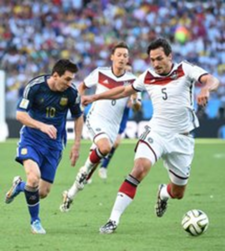
\includegraphics[width=0.6\linewidth]{soccer}
    \caption{德国足球}
\end{figure}

    德国国家队被誉为世界上最有名及最成功的国家足球队之一,德国也是目前为止唯一一个包揽男、女足世界杯冠军的国家。曾经四次夺得世界杯(1954年,1974年,1990年,2014年),仅次于巴西,由1954年开始从未缺席过世界杯决赛圈。德国亦曾经三次夺得欧洲国家杯冠军(1972年,1980年,1996年),是夺得最多欧洲国家杯冠军的球队。德国足球的传统是身体力量与技术的结合,可以适应各种技战术打法的全能足球风格。被称为绿茵场上的"德国战车"。 

\subsection{德国足球强大的原因}
\begin{figure}[htb]
    \centering
    
\includegraphics[width=0.6\linewidth]{victory}
    \caption{胜利}
\end{figure}

    大刀阔斧的改革:2001年,共同商讨决定,所有的德甲俱乐部必须要对青训营进行投资,使得其成为年轻人最好的平台. 
    
    德国足球另一个成功的因素就是这个国家完备的球探网络。总计有超过300家球探中心,去搜索和培养年轻天才。 
    
    重视球员的教育水平,好的教育令球员们不仅在足球领域之外获得了更有质量的生活,同时也让他们学会了更多技巧,获得了更多机会。他们可以更好地理解教练员和管理团队的战术和建议,更快的传递信息,更重要的是,在教室里学到的知识可以让他们的大脑更加丰富,更有利于做决定。 

\subsection{德国足球背后的文化}
\begin{figure}[htb]
    \centering
    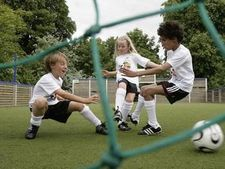
\includegraphics[width=0.6\linewidth]{kidssoccer}
    \caption{儿童足球}
\end{figure}

\subsection{中国乒乓球}
\begin{figure}[htb]
    \centering
    \includegraphics[width=0.6\linewidth]{tableteniss}
    \caption{乒乓}
\end{figure}

    中国乒乓球队成立于1952年,1959年乒乓球运动员容国团为中国夺得了第一个世界冠军。第26届世界乒乓球锦标赛上中国分别获得男女单打冠军,中国队也拿下了男子团体冠军。从这个时候开始,中国乒乓运动开始在中国长盛不衰。至2005年,共获冠军143.5枚,其中世锦赛100. 5枚,世界杯赛27枚,奥运会16枚。而且已有三次包揽世锦赛全部7个金杯,两次包揽奥运会全部4枚金牌。

\subsection{中国乒乓强大的原因}
\begin{figure}[htb]
    \centering
    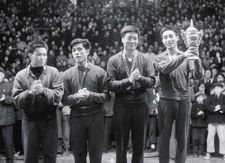
\includegraphics[width=0.6\linewidth]{award}
    \caption{中国乒乓}
\end{figure}

    历史原因:新中国成立后,毛泽东主席号召“发展体育运动,增强人民体质”,乒乓球因为对场地要求不高,简便易行所以在全国开展得比较好。1959年乒乓球运动员容国团为中国夺得了第一个世界冠军。此后,乒乓球受到国家与人民的喜爱。 
    适合中国的国情:乓球运动开展的条件宽松,可参与性强。男女老少都能打,天南海北都能打,室内室外都能打,有钱没钱都能打。它没有直接的身体对抗,自己可控制运动量,非常有利于普及。 
    出色的运动员与开展的普遍性:现在中国几乎每个公园都有乒乓球台,几乎所有学校都有常规训练的乒乓球队,并且乒乓球冠军都很知名。中国有1000万人经常参加乒乓球比赛,3亿人会打乒乓球。多年来中国选手一直在乒乓球项目中有着极为出色的表现,多年来中国乒乓球队一直以“梦之队”的姿态出现在奥运赛场上,乒乓球项目也是中国代表团最为稳固的夺金点之一。

\subsection{中国乒乓球背后的文化}
\begin{figure}[htb]
    \centering
    \includegraphics[width=0.6\linewidth]{tableteniss in school}
    \caption{校园乒乓}
\end{figure}

    自1959年容国团为新中国赢得第一个世界冠军以来,乒乓球运动极大的增进了民族凝聚力、增强民族自信心和自豪感。中国乒乓球运动员在赛场上的表现,体现了中国运动员,勤奋刻苦、善于创新。在中国,乒乓球运动的口号“人生能有几回搏”,“胸怀祖国,放眼世界”, “胜了从零开始,败了打翻身仗”

\subsection{结语}
    通过以上介绍,想必你们一定对中国乒乓球与德国足球有了基本的认识。无论是中国乒乓球还是德国足球都反应了一个民族的体育精神和民族文化。通过一项体育运动我们可以清楚认识一个伟大国家的民族性格和民族信心。



\section{交通}
    交通工具改善了我们的生活。让我们这个地球变得就像一个大家园,紧紧相连,假若没有交通工具,也许有一些人一辈子都和家人见不到面。远在天南地北、千里万里的新鲜果品,快速运到各地使人们尝鲜。上学、上班、旅游、物资运输,传递信息,可以风雨无阻。免去风吹日晒雨淋的痛苦。身体不便的人,也能到处活动。这些都要用到交通工具,交通工具是我们生活中不可缺少的一部分。可见,交通工具多么重要。而作为中德工程师学院的一员,当我们去德国旅游或是读书,到达德国的第一步就是先要想办法去到我们的旅馆,所以事先熟悉德国的交通就显得十分重要。
    随着时代的高速发展,各国之间的经济差距慢慢变小,而交通工具的差异也在这其中被慢慢消减。所以,现在中德两国出行时的交通工具其实也是大致相似的。

\subsection{公共交通}
\begin{figure}[htb]
    \centering
    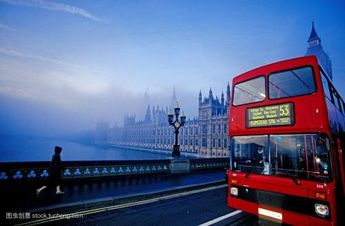
\includegraphics[width=0.6\linewidth]{bus}
    \caption{公交车}
\end{figure}

    “公共自行车,公交车,地铁,城市轻轨,出租车,滴滴” 

    公交线路大都覆盖了城市的各个中心区,选择公共交通出行可以大大方便我们的生活,不论是去上班,学习还是旅游。除此之外,选择公共交通出行还更加的省钱;我们可以利用坐车的时间听听歌,看看书,放松自己;并且可以把注意力完全防到城市的风景中,了解城市的动态;除此之外,还能够有更多的时间和心爱的人在一起,当然,前提条件是你们要刚好顺路。 
  
    不过中国和德国不同的一点是,中国拥有大量的共享单车以及滴滴打车的出行方式。 这主要是因为中国手机支付方式的流行,只要用支付宝或是微信扫一扫,就能解锁共享单车。 更为方便的是,只要你手机里有“滴滴打车”APP或是微信,在简单的注册后,就能一键叫到出租车,十分方便。

\subsection{个人出行}

\begin{figure}[htb]
    \centering
    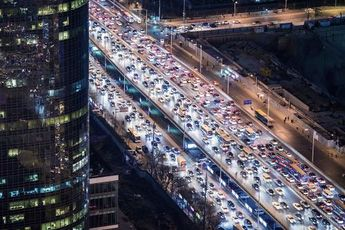
\includegraphics[width=0.6\linewidth]{night piece}
    \caption{自驾车}
\end{figure}

    “步行,自行车,电动车,私家车” 

    自驾出行往往更为的便捷,可以随时随地出门,想去哪儿去哪儿,不用受到公交出行固定时间的限制;而且自驾出行更为的舒适,可以拥有自己的一片空间。 
    
    但是现在的城市中交通大都十分堵塞,尤其在早高峰与晚高峰期间,平常只要两个小时的路程,甚至要花上三个小时才能到目的地。所以并不推荐。

\subsection{长途}
\begin{figure}[htb]
    \centering
    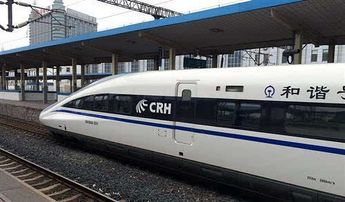
\includegraphics[width=0.6\linewidth]{railway}
    \caption{高铁}
\end{figure}

    “高铁,高速公路,火车,飞机” 

    近些年快速发展的高铁可以说完全改变了人们的出行方式。举个例子,在中国,十年前从杭州到北京坐火车需要花上一天两夜,但现在,因为有了高铁,仅需六个小时。 
    
    高铁以其高速的运行速度,快速的赢得了人们的青睐。

\subsection{结语}
    在中国或是德国我们都有许多的出行方式可以选择。所以更为重要的是在出行前做好选择,使用正确的最舒适的方式。



\subsection{艺术}
    艺术是反应过去时代文化和人们对地域环境影响下形成的文化标志之一,在历史的长河中,各个地域、各个民族都形成了风格迥异的艺术文化。如果你对中德两国近代的艺术方面感兴趣的话,不妨点击条目看看。

    如果你曾经切实聆听过德国的传统音乐以及中国的传统音乐,你会发现无论是旋律还是音调都有相当的差异,接下来我将从传统音乐的文化,著名作曲家,现状以及乐器方面展示差异产生的原因。

\subsection{中国传统音乐文化}
\begin{figure}[htb]
    \centering
    
\includegraphics[width=0.6\linewidth]{chinese instruments}
    \caption{中国古典乐器}
\end{figure}

    中国传统音乐,文献一般追溯到黄帝时代,据考古发现,中国音乐可追溯至7000多年前,中华民族在几千年的历史长河中,创造了丰富的音乐文化。同时从孔子传六艺到唐代的胡琴再到近代的西方音乐,中国音乐又在吸收外来音乐要素的过程中不断充实发展。中国素号“礼乐之邦”,古代音乐在人格养成、文化生活和国家礼仪方面有着很重要的作用和地位。通俗音乐是中国音乐的方式,即旋律为主,五声音阶为主,才能受到最多人的喜爱。 

\subsection{中国著名传统音乐家及代表作}
\begin{figure}[htb]
    \centering
    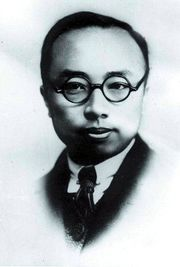
\includegraphics[width=0.6\linewidth]{liutianhua}
    \caption{刘天华}
\end{figure}
    刘天华-《良宵》,《光明行》,《病中吟》 

    华彦钧-《二泉映月》,《听松》,《大浪淘沙》 

\subsection{中国传统音乐现状}
\begin{figure}[htb]
    \centering
    
\includegraphics[width=0.6\linewidth]{national theater}
    \caption{国家大剧院}
\end{figure}

    中国音乐教育有着庞大的教学体系,但是当代音乐教学出现一种严重的西化现象,大多数学生更加了解西方的音乐文化和乐器,而对自己国家的音乐文化和乐器却十分陌生,甚至有部分学生对我国的戏曲产生厌烦的情绪,表示无法接受这种艺术,其艰涩难懂也是很大一部分原因,再加上快节奏的生活,很少有学生能够沉下心来静静的欣赏传统音乐的魅力所在。 
    
    中国有非常多的剧院数量(超过2000家),但是出名的歌剧院并不多。有名的歌剧院有上海大剧院、国家大剧院、广州大剧院等。 

\subsection{德国传统音乐文化}
\begin{figure}[htb]
    \centering
    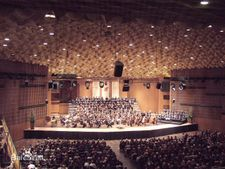
\includegraphics[width=0.6\linewidth]{music festival}
    \caption{贝多芬音乐节}
\end{figure}
    
    德国以音乐闻名于世,它是世界上著名的音乐之乡。 
    
    德意志民族是一个热爱音乐且极具音乐天赋的民族,它在音乐方面的成就无与伦比,世界上几乎没有哪一个国家在其历史发展过程中,能像德国一样造就了如此之多的音乐名家。 巴赫和亨德尔是德国17世纪最杰出的作曲家;海顿、莫扎特和贝多芬三人被称为维也纳最杰出的古典音乐大师;作为德国歌曲之王的舒伯特与舒曼则是19世纪德国浪漫派音乐的杰出代表;19世纪下半叶,决定德国乃至欧洲音乐发展道路的中心人物是瓦格纳;此外还有勃拉姆斯、勋伯格、米德米特等音乐名家他们也为德国及世界音乐发展作出了重要贡献。 
   
    德国至今有许多艺术节或音乐团体就是为纪念这些艺术大师而专设的。如波恩国际贝多芬节、拜罗伊特瓦格纳文化节、献身巴赫音乐的盖兴教堂唱诗班和国际巴赫协会及不定期举行的巴赫文化节等等。 

\subsection{德国著名传统音乐家及代表作}

\begin{figure}[htb]
    \centering
    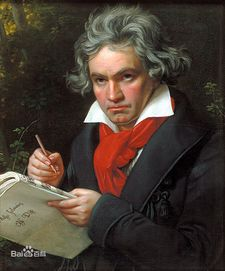
\includegraphics[width=0.6\linewidth]{beethoven}
    \caption{贝多芬}
\end{figure}

    贝多芬-命运交响曲, 第九交响曲, 威灵顿的胜利等 
   
    理查·施特劳斯-蓝色多瑙河, 阿尔卑斯交响曲, 家庭交响曲等 
   
    约翰·塞巴斯黛安·巴赫-B小调弥撒等 

\subsection{德国传统音乐现状}
\begin{figure}[htb]
    \centering
    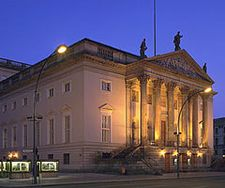
\includegraphics[width=0.6\linewidth]{national theater02}
    \caption{德国国家歌剧院}
\end{figure}

    今日德国的年轻一代,每两个人中就有一人会弹奏一种乐器。年轻人听音乐的兴趣始终胜于看电视 。 
    
    德国有121座歌剧院(德国国家歌剧院,巴伐利亚国家歌剧院,德累斯顿森珀歌剧院等)、146个职业乐队,它们全都由国家资助。 
  
    德国每年售出的本国和国际上生产的唱片、磁带和激光唱片达2.4亿张。德国8千多万人口;合唱团就有4万个,还有2.5万个业余或专业乐团和舞蹈团 。 

\subsection{传统音乐上的乐器差异}
\begin{figure}[htb]
    \centering
    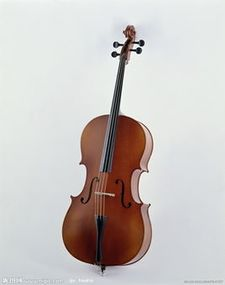
\includegraphics[width=0.6\linewidth]{cello}
    \caption{大提琴}
\end{figure}

    德国古典音乐的乐器主要包括钢琴,风琴,大提琴,小提琴等。 
    
    中国古典音乐所使用的乐器主要包括二胡,鼓,琵琶,萧等。 

\subsection{结语}
    传统的文化与传统的音乐家奠定了传统音乐的风格,而不同地区间不同的乐器则确定了传统音乐的形式与格局,两者之间的共同作用产生了中德音乐文化的差异。


\section{卫生}
    卫生是疾病预防和保护,促进和加强健康的科学。 “卫生”一词来自希腊语,意思是“健康服务艺术”。 卫生或个人卫生措施的目的是保持和改善个人(个人卫生)和社会(一般卫生)的表现和福祉。 卫生是预防疾病和健康损害的所有措施的总和,其中一个主要重点是预防传染病。

\subsection{日常生活中的卫生}
    在日常生活中,必须遵守一些卫生措施,以保护自己和他人免受细菌,病毒和真菌的感染,并特别预防疾病。日常卫生的范围从彻底的洗手到定期清洁表面和物体。付款通常在中国以现金支付、支付宝或微信支付。使用电子支付的方式能减少了与账单的联系。
    \begin{figure}[htb]
        \centering
        
\includegraphics[width=0.6\linewidth]{Mundschultz}
        \caption{通过戴口罩防止病菌入侵}
    \end{figure}

\subsection{厕所的卫生}
    在卫生室中,清洁和卫生尤其重要,因为特别是在浴室和厕所中,细菌传播的风险很大。

    对于卫生设施的清洁/消毒,有各种各样的洗涤剂/消毒剂用于各自的应用领域(例如厕所清洁剂,浴室清洁剂,脱模剂等)。

    顺便说一句,省钱是不合适的 - 只有经常使用合适的清洁/消毒剂清洁的人才能保护自己和他人免受感染和疾病。不要忘记门把手,因为他们在没有洗手的情况下使用厕所后会被触摸。为了将任何细菌从厕所转移到浴室,应始终使用不同的清洁用具用于不同的区域。在清洁/消毒后将它们洗涤或丢弃。应始终按照清洁/消毒剂的说明进行清洁/消毒,并始终佩戴橡胶手套。

    德国的每个厕所都配有一个皂液器。因为通过使用细菌/病原体在厕所后最小化。
    \begin{figure}[htb]
        \centering
        
\includegraphics[width=0.6\linewidth]{washhands}
        \caption{如何正确洗手}
    \end{figure}

\subsection{马桶的卫生}
    中国厕所更卫生,因为它们不与座位接触。卫生纸在德国的厕所中被直接冲走,而在中国,它通常被丢弃在垃圾箱中。 在中国,卫生纸在公共厕所中不常见,而在德国,厕所里没有卫生纸是不可想象的。

    \begin{figure}[htb]
        \centering
        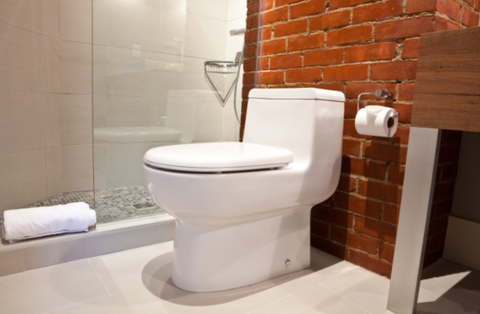
\includegraphics[width=0.6\linewidth]{deutsche Toilette}
        \caption{德国马桶}
    \end{figure}

    \begin{figure}[htb]
        \centering
        \includegraphics[width=0.6\linewidth]{chinesische Toillete}
        \caption{中国马桶}
    \end{figure}